\subsection{Case Study}\label{sec:case}

We conduct case study on the \pt{} dataset to demonstrate the visualization quality of $\avats$. The observations are similar for the other datasets and we omit their results for conciseness.

\begin{figure*}[t]
	\centering
	\includegraphics[width=0.85\textwidth]{pictures/case_study_icde/case_study_detail.pdf}
	\trim
	\vspace{-2mm}
	\caption{Case study of the visualization quality of $\avats$ for two detail regions.}
	\label{fig:detailview}
	\trim \trim
\end{figure*}

\begin{figure*}
	\centering
	\small
	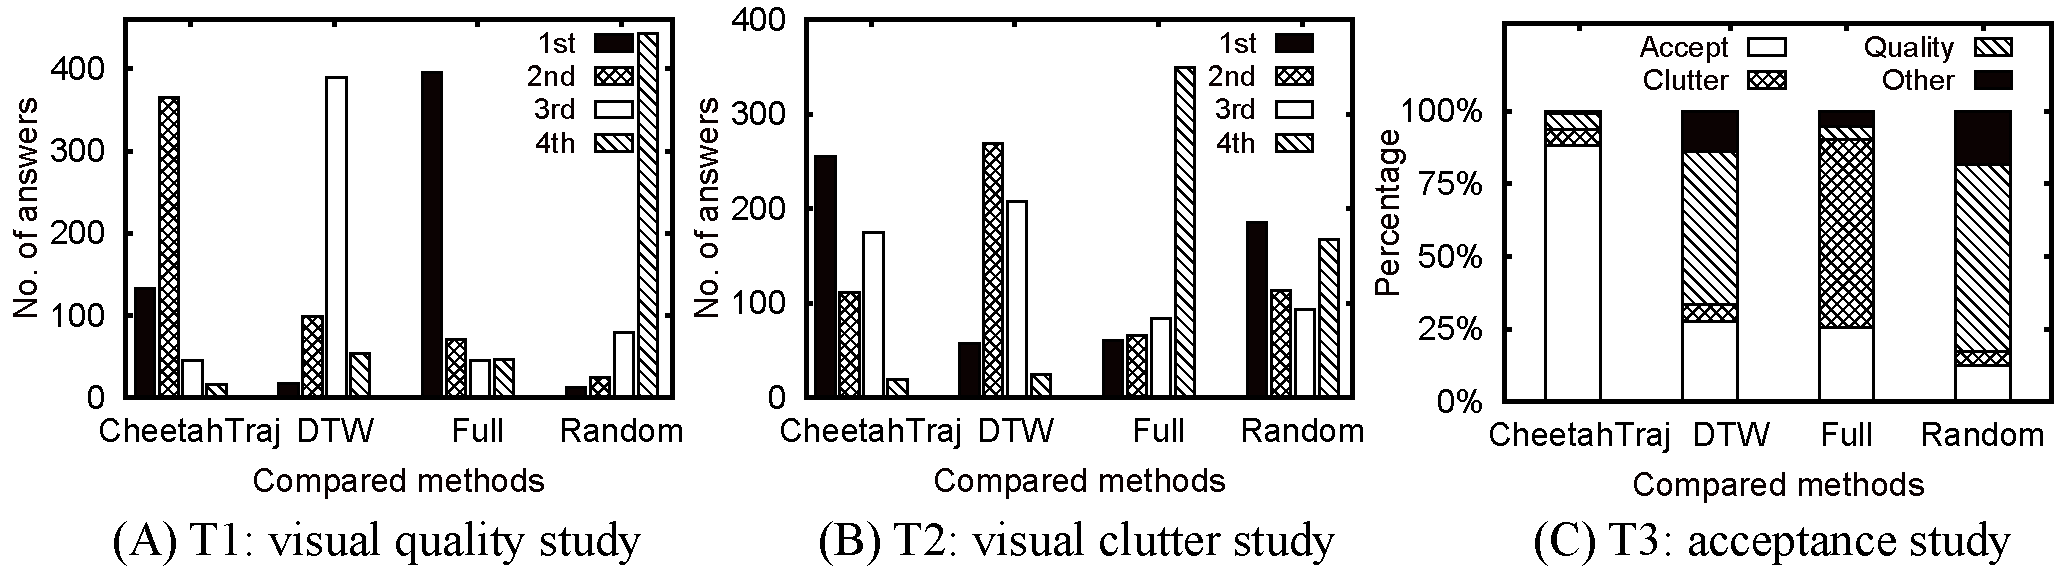
\includegraphics[width=1.3\columnwidth]{pictures/user_study/user_study.pdf}  
	\trim \trim
	%\vspace{-3mm}
	\caption{User study results of different visualization methods.} 
	\label{fig:userstudy}
	\trim \trim
\end{figure*}



\subsubsection{Overview visualization}

We illustrate the visualization results of different methods for the entire \pt{} dataset in Figure~\ref{fig:overview}.

\stitle{Good visual quality for overview}
At zoom level 11, Figure~\ref{fig:overview}(A) is the visualization result of $\mathsf{Full}$ on the \pt{} dataset.
With a sampling rate $\alpha \!=\! 1\%$, Figures~\ref{fig:overview}(B), (C) and (E) are the visualizations produced by $\mathsf{Random}$, $\mathsf{DTW}$,
and $\avats$, respectively. Comparing with Figure~\ref{fig:overview}(B) and (C), it is obvious that Figure~\ref{fig:overview}(E) is more similar to Figure~\ref{fig:overview}(A). In particular, Figure~\ref{fig:overview}(E) not only preserves the overall visual structure of the entire region but also keeps the details of cities that are far from the center (marked by the dashed cycles). However, the details of these cities are lost in Figure~\ref{fig:overview}(B) as $\mathsf{Random}$ mostly selects trajectories in the dense region. $\mathsf{DTW}$ in Figure~\ref{fig:overview}(C) preserves more details than $\mathsf{Random}$ in the sparse regions as it considers diversity in trajectories but its visualization quality is still inferior compared with $\avats$ in Figure~\ref{fig:overview}(E).

\stitle{Good visual quality under different sampling rates}
Figure~\ref{fig:overview}(D) and (E) are the visualizations produced by $\avats{}$ with a sampling rate of $0.1\%$ and $1\%$, respectively. We can make two observations: (i) the larger the sampling rate, the better the visual quality, i.e., Figures~\ref{fig:overview}(E) is more similar to Figure~\ref{fig:overview}(A) than Figure~\ref{fig:overview} (D); (ii) the visualization of $\avats$ with a sampling rate of $0.1\%$ (i.e., Figure~\ref{fig:overview}(D)) looks more appealing than the visualizations of $\mathsf{Random}$ and $\mathsf{DTW}$ with a sampling rate of $1\%$ (i.e., Figure~\ref{fig:overview}(B) and (C)) as Figure~\ref{fig:overview}(D) better preserves the structures in Figure~\ref{fig:overview}(A).



\stitle{Color encoding effectively mitigates visual clutter} At zoom level 11 and with a sampling rate of $1\%$, Figures~\ref{fig:overview}(E) and (F) are the visualizations produced by our $\avats$ and $\cavats$ (i.e., enabling color encoding), respectively.
Visual clutter is severe for $\mathsf{Full}$ (i.e., Figure~\ref{fig:overview}(A)) and $\avats$ (i.e., Figure~\ref{fig:overview}(E)) as many pixels are visualized for the dense region in the center, which makes it difficult to identify the main routes. The visualization of $\cavats$ in Figure~\ref{fig:overview}(F) alleviates this problem by encoding more representative trajectories with warmer color, making it easier to identify some main routes than Figure~\ref{fig:overview}(A) and (E).

%\vspace{1mm}
\subsubsection{Detail visualization}\label{sec:detail}




We analyze the visualizations produced by different methods for small areas with details by investigating two regions of interest in the \pt{} dataset in Figure~\ref{fig:detailview}.

%We next present the effectiveness of our proposals with detail views by investigating two regions of interest in \pt{}, the dense region B and the sparse region C(shown as in Figure~\ref{fig:detailview}(8)).

%$\mathsf{Full}$
%$\mathsf{DTW}$
%$\mathsf{Random}$

\stitle{Reduce visual clutter and preserve micro structures for dense region} At zoom level 15, region B in Figure~\ref{fig:detailview}(A) is the center of Porto and has the highest concentration of trajectories. Therefore, $\mathsf{Full}$ suffers from severe visual clutter and it is difficult to identify the road networks in Figure~\ref{fig:detailview}(B1).  $\mathsf{Random}$ and $\mathsf{DTW}$ in Figure~\ref{fig:detailview}(B2) and (B3) reduce the visual clutter to some extent by sampling some trajectories. $\avats$ in Figure~\ref{fig:detailview}(B4) is more successful in reducing the visual clutter of $\mathsf{Full}$ and allows to identify a much larger number of routes. In addition, $\avats$ preserves more micro structures of the trajectories than $\mathsf{Random}$ and $\mathsf{DTW}$, e.g., the circular route in the dashed circular region.

% and causes serious visual clutter, as visualized in Figure~\ref{fig:detailview}(B1).
%For example, the circular structures of the main route(shown as the dashed circular region in Figure~\ref{fig:detailview}(B1)) is unclear.
%$\localavats$ alleviates the visual clutter by preserve the $1\%$ trajectories of the total regions but the clutter is still serious. Furthermore, $\avats$ performs better than $\localavats$ by preserving less trajectories and reduce the visual clutter.


\stitle{Preserve overall layout for sparse region}
At zoom level 14, region C in Figure~\ref{fig:detailview}(A) contains the city of Casino Espinho and has fewer trajectories than the dense region in the center. In this case, the sampling methods need to keep the overall layout of the trajectories  to provide good visualization quality. Compared with $\mathsf{Full}$ in Figure~\ref{fig:detailview}(C1), $\mathsf{Random}$ and $\mathsf{DTW}$ in Figure~\ref{fig:detailview}(C2) and (C3) fail to meet this requirement as they do not show any trajectory for areas far from the city, e.g., in the dashed circle. This makes their entire visualization layout very different from $\mathsf{Full}$. In contrast, $\avats$ in Figure~\ref{fig:detailview}(C4) preserves the trajectories in areas far from the city and has a overall layout similar to $\mathsf{Full}$.

%Region C includes the city of Casino Espinho at zoom level 14, which contains less trajectories than the center of Porto as the visualization result of full dataset shown in Figure~\ref{fig:detailview}(C1).
%Given fix sampling rate $\alpha=1\%$, Figure~\ref{fig:detailview}(C2) indicates the visualization of $\localavats$. This visualization result misses a lot if detail information in this region, because the fix sampling rate preserves too few trajectories which is difficult to guarantee the visual quality.
%While $\avats$ in Figure~\ref{fig:detailview}(C3) performs much better than $\localavats$ as the sampling rate is automatically adjusted to according to the visual quality. In this visualization, the trajectory sketch of Casino Espinho is almost the same as it in Figure~\ref{fig:detailview}(C1), the visualized result of full dataset.

%To sum up, the case study shows that $\avats$ effectively mitigates visual clutter with sampling and color encoding. With the quality-aware $\vatss$ algorithm, $\avats$ also provides better visualization quality than $\mathsf{Random}$ and $\mathsf{DTW}$ by preserving the micro structures and overall layout of full visualization.

To sum up, the case study shows that $\avats$ effectively mitigates visual clutter. In addition, $\avats$ also provides better visualization quality than $\mathsf{Random}$ and $\mathsf{DTW}$ by preserving the micro structures and overall layout of full visualization.
